\phantomsection\numberedsection{RF1 Gestión de Cuentas}

\subsection*{Descripción}
El sistema muestra un informe detallado con la información de la cuenta, incluyendo la información del
nombre de la cuenta, fecha y hora de creación, número de productos y tamaño utilizado de almacenamiento
en bytes, número de categorías de productos y assets, número de atributos de usuario
creados y el número de relaciones creadas.

\vspace{0.15cm}

\textbf{Pre-condición}\par
El usuario ha iniciado sesión en Mini PIM y es la cuenta Owner.\par
\vspace{0.15cm}

\textbf{Post-condición}
\begin{itemize}
    \item Caso de éxito: El sistema muestra el informe detallado de la cuenta.
    \item Caso de error: El sistema notifica al usuario el resultado al crear el informe: exitosa o fallida.
\end{itemize}

\textbf{Prioridad:}
Baja
\vspace{0.15cm}

\textbf{Autor: }
Janine Olegario\par
\vspace{0.15cm}

\textbf{Control de cambios: } Versión 1: Definición del caso de uso

\numberedsubsection{Escenario principal}
\begin{enumerate}
    \item El usuario selecciona la opción \enquote{Cuenta} desde el \textit{Dashboard}.
    \item El sistema genera un informe con los datos de la cuenta del usuario
    \item El sistema muestra al usuario el informe completo con los siguientes datos:
        \begin{itemize}
            \item Nombre de la cuenta
            \item Fecha y hora de creación de la cuenta
            \item Número de productos de la cuenta
            \item Tamaño utilizado de almacenamiento en bytes
            \item Número de categorías de productos
            \item Número de atributos de usuario creados
            \item Número de relaciones creadas.
        \end{itemize}
\end{enumerate}

\numberedsubsection{Escenarios alternativos}
\begin{description}
    \item[3.a] El sistema no encuentra productos que coincidan con la búsqueda por SKU o label.
    \begin{enumerate}
        \item[3.a.1] El sistema muestra un mensaje indicando que no hay productos que coincidan con los criterios de búsqueda.
    \end{enumerate}

    \item[*.a] El usuario cancela la búsqueda sin ingresar un SKU o un label.
    \begin{enumerate}
        \item[*.a.1] El sistema muestra la lista completa de productos sin aplicar filtros.
    \end{enumerate}

    \item[5.a] No hay productos registrados en el sistema.
    \begin{enumerate}
        \item[5.a.1] El sistema muestra un mensaje indicando que no hay productos disponibles para mostrar.
    \end{enumerate}
\end{description}

\numberedsubsection{Casos de Prueba}
\underline{Escenario: Principal}\par
\vspace{0.15cm}
\textbf{Dado} que el usuario ha iniciado sesión en su cuenta en Mini PIM,\par
\textbf{Cuando} selecciona la opción de \enquote{Productos} en el menú principal,\par
\textbf{Entonces} el sistema carga y muestra la lista de productos en un \textit{DataGrid} con todos los atributos visibles.\par
\vspace{0.20cm}

\underline{Escenario: Alternativo 3.a}\par
\vspace{0.15cm}
\textbf{Dado} que el usuario intenta buscar un producto mediante SKU o label,\par
\textbf{Cuando} no hay productos que coincidan con los criterios de búsqueda,\par
\textbf{Entonces} el sistema muestra un mensaje indicando que no hay productos que coincidan.\par
\vspace{0.20cm}

\underline{Escenario: Alternativo *.a}\par
\vspace{0.15cm}
\textbf{Dado} que el usuario ha abierto la sección de productos,\par
\textbf{Cuando} cancela la búsqueda sin ingresar un SKU o label,\par
\textbf{Entonces} el sistema muestra la lista completa de productos sin aplicar filtros.\par
\vspace{0.20cm}

\underline{Escenario: Alternativo 5.a}\par
\vspace{0.15cm}
\textbf{Dado} que el usuario ha iniciado sesión en Mini PIM,\par
\textbf{Cuando} selecciona la opción de \enquote{Productos} y no hay productos registrados en el sistema,\par
\textbf{Entonces} el sistema muestra un mensaje indicando que no hay productos disponibles para mostrar.\par
\vspace{0.20cm}


\numberedsubsection{Bocetos}
\begin{figure}[H]
    \includegraphics[width=1\linewidth]{mockups/RF2- Gestión General de Productos (listado).png}
    \caption{Listado de Productos}
   \end{figure}
\vspace{1.0cm}

\begin{figure}[H]
    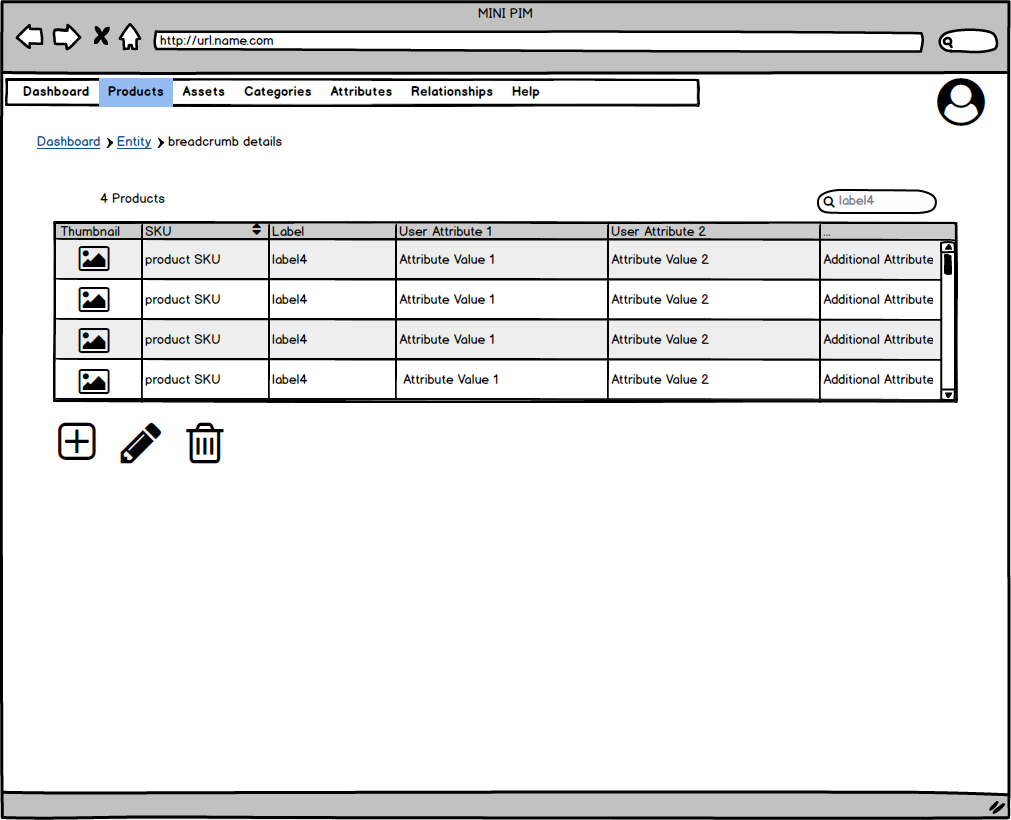
\includegraphics[width=1\linewidth]{mockups/RF2- Gestión General de Productos (listado por búsqueda).png}
    \caption{Listado de Productos con búsqueda filtrada por label}
   \end{figure}
\vspace{1.0cm}

\newpage %Inicia en una nueva página otro caso de uso